
\documentclass[11pt]{article}
\usepackage[a4paper,top=2.2cm,bottom=2.4cm,left=3.3cm,right=3.3cm,headheight=14pt]{geometry}
\usepackage[T1]{fontenc}
\usepackage{mathpazo}
\usepackage{amsmath,amssymb}
\usepackage{microtype}
\usepackage{graphicx}
\usepackage{booktabs}
\usepackage{array}
\usepackage{xcolor}
\usepackage{fancyhdr}
\usepackage{titlesec}
\usepackage{caption}
\usepackage{listings}
\usepackage[authoryear,round]{natbib}
\usepackage[pagebackref]{hyperref}
\definecolor{linkblue}{RGB}{90,110,170}
\hypersetup{colorlinks=true,linkcolor=linkblue,citecolor=linkblue,urlcolor=linkblue}
\renewcommand*{\backref}[1]{}\renewcommand*{\backreftwosep}{, }\renewcommand*{\backreflastsep}{, }
\renewcommand*{\backrefalt}[4]{\ifcase #1 \or [p#2]\else [p#2]\fi}
\pagestyle{fancy}\fancyhf{}
\fancyhead[L]{\textsc{Preprint}}\fancyhead[R]{\thepage}
\renewcommand{\headrulewidth}{0.6pt}
\titleformat{\section}{\normalfont\Large\bfseries}{\thesection}{1em}{}
\titleformat{\subsection}[runin]{\normalfont\large\bfseries}{}{0pt}{}
\titlespacing*{\subsection}{0pt}{2.2ex plus .5ex}{0pt}
\newcommand{\subsec}[1]{\par\vspace{1.6ex}\noindent{\large\bfseries #1}\par\vspace{0.8ex}\noindent\ignorespaces}
\captionsetup{font=small,labelfont=bf,labelsep=colon}
\lstset{basicstyle=\ttfamily\small,columns=fullflexible,keepspaces=true,showstringspaces=false,xleftmargin=0pt,aboveskip=1.2ex,belowskip=1.2ex}
\newcommand{\code}[1]{\texttt{#1}}
\setlength{\parindent}{1.4em}
\setlength{\parskip}{0pt}
\begin{document}
\thispagestyle{fancy}

\noindent{\fontsize{22}{27}\selectfont\bfseries Early Warning from Public Data:\\An Interpretable, Calibrated\\School-Level Model of First-Year\\College Outcomes in Indiana\par}
\vspace{0.6ex}
\noindent{\itshape by Othniel Iyassa Sa'anga}

\vspace{2.2ex}
\noindent\textbf{Abstract} Weak first-year college outcomes cost students time and money, yet high schools learn about them only after a cohort has finished its first college year. We present an interpretable, calibrated early-warning model that predicts, for each Indiana public high school, the mean first-year credits and grade point average of its graduates who enroll at an Indiana public college, using only public school-level signals observable before those students reach college: grade 7/8 state mathematics results, grade 11 SAT mathematics results, the grade in which students pass Algebra~I, whether advanced mathematics and calculus are offered, AP exam passing, and dual-credit earning. The model is estimated on the graduating class of 2023 and evaluated on the class of 2024, which it never saw. A weighted linear model explains 59\% of between-school variation in first-year credits (95\% CI 45\%--68\%) and 56\% in GPA, matches gradient-boosted trees, and outperforms each school's own prior-cohort outcome. Information available by grade~9 explains 45\% of variation in credits and grade 11 SAT mathematics raises this to 58\%. Predictions are well ordered but slightly over-dispersed (calibration slope 0.87) and miss a statewide level shift. A failure audit shows systematic GPA errors at small, rural, high-poverty and virtual schools, and school poverty alone predicts GPA about as well as the lever set. Mathematics remediation is too rare and too heavily suppressed to model. The panel, code, model card and an interactive school map are openly released.

\section{Introduction}

Indiana publishes, for every high school, how its graduates fare at Indiana public colleges: how many enroll, how many need remediation, and the average credits and GPA they earn in the first year \citep{che2026}. These reports arrive late by construction. A cohort's first-year outcomes are released about two years after it graduates, roughly five years after it sat the grade 8 state test and two years after its grade 11 SAT. By the time a high school learns that its graduates accumulate credits slowly, several more cohorts have passed through the same mathematics pathway. The scale of the problem is not small: 36\% of the class of 2024's Indiana public college enrollees earned fewer than 24 credits in their first year, the pace needed to finish a bachelor's degree in four years or an associate degree in two.

Early-warning systems for high school graduation are well established. The Chicago on-track indicator showed that a small set of ninth-grade signals forecasts graduation well \citep{allensworth2005}, and the precision and sensitivity of dropout predictors have been reviewed systematically \citep{bowers2013}. The college side of the transition has received less attention as a forecasting problem. A large literature studies its parts: test-based placement misclassifies many students \citep{scottclayton2012}; long developmental sequences lose students \citep{bailey2010}; college mathematics readiness depends on the level and timing of high school mathematics \citep{adelman2006,long2009}; acceleration into Algebra~I is not uniformly beneficial \citep{clotfelter2015,domina2015}; and dual enrollment is associated with later degree attainment \citep{an2013}. What is missing is a transparent tool that combines these signals, at the level at which a state actually publishes them, into a calibrated forecast for each school, early enough to act on and with its failures documented.

This paper builds and audits such a tool for Indiana. We ask three questions. First, how well do public school-level signals predict a school's first-year college outcomes for a graduating cohort that the model has never seen? Second, how early is the warning available: by grade~9, by grade~11, or only at graduation? Third, where does the model fail, and does it fail evenly across kinds of schools? The design follows reporting conventions from clinical prediction modeling \citep{collins2015,steyerberg2019}: a temporal hold-out rather than only cross-validation, calibration given the same weight as discrimination \citep{vancalster2019}, explicit benchmarks, and a model card \citep{mitchell2019}.

The contribution is threefold. Substantively, we show that most of the predictable variation in school-level first-year outcomes is visible two years before graduation and that a linear model is sufficient. Methodologically, we provide a complete, reproducible pipeline that aligns four graduating cohorts with assessments that changed scale (ISTEP+ to ILEARN), a cancelled test year (2020), a new state SAT (from the class of 2023) and biennial federal course data. Practically, we release the panel, every intermediate file with cryptographic provenance, and an interactive map. Section~\ref{sec:background} positions the work. Section~\ref{sec:data} describes the data and pipeline, Section~\ref{sec:methods} the models and validation design, and Section~\ref{sec:results} the results. Section~\ref{sec:discussion} discusses use and limitations, and Section~\ref{sec:conclusion} concludes.

\section{Background and related work}\label{sec:background}

This section summarizes the three bodies of work the model draws on and clarifies what is new. The aim is not a comprehensive review but a statement of the information structure: which signals are observed, when, and at what level of aggregation.

\subsec{Early-warning indicators in secondary school}
Early-warning indicators turn routinely collected student records into forecasts of a later outcome. The ninth-grade on-track indicator combines course failures and credits into a single flag that predicts graduation with high accuracy \citep{allensworth2005}. \citet{bowers2013} compare 110 dropout flags on precision and sensitivity and find that many widely used flags perform little better than chance, which is why we report precision and recall against explicit baselines. These systems operate on student records inside a district. Our setting is different: the outcome is observed only in aggregate, after a delay, and the predictors are public school-level statistics. The appropriate analogue is therefore a school-level screening tool, not a student-level risk score.

\subsec{College readiness and mathematics course-taking}
Mathematics is the most common barrier in the transition to college. Remedial placement based on a single test misclassifies many students \citep{scottclayton2012}, and students referred to multi-level developmental sequences frequently never complete them \citep{bailey2010}. The intensity of high school mathematics, particularly courses beyond Algebra~II, predicts degree completion \citep{adelman2006}, and differences in high school course-taking account for a large share of gaps in college mathematics readiness \citep{long2009}. Timing matters in both directions: pushing more students into Algebra~I in grade 8 lowered later mathematics achievement in some districts \citep{clotfelter2015} and did not raise advanced course-taking in California's statewide effort \citep{domina2015}. Dual enrollment is associated with higher degree attainment, including for low-income students \citep{an2013}. These findings motivate the lever set: grade 8 mathematics, the grade at which Algebra~I is passed, the availability of advanced mathematics and calculus, AP exam passing and dual credit.

\subsec{Prediction-model reporting and calibration}
A forecast used for screening must be judged on more than correlation. The TRIPOD statement \citep{collins2015} sets out what a prediction-model report should contain, including validation design and calibration. Calibration (whether predicted values match observed values in level and spread) is often neglected even though it determines whether predictions can be used as absolute targets \citep{vancalster2019}. The calibration slope and intercept go back to \citet{cox1958}. We adopt these tools for a continuous school-level outcome and add a failure audit by school type, in the spirit of model cards \citep{mitchell2019}.

\subsec{What is new here}
Indiana's college-going reports are widely used descriptively, but we are not aware of a published model that forecasts them from earlier public school-level signals with a temporal hold-out, calibration and a subgroup audit. The contribution is the forecasting framing, the cohort alignment that makes it possible, and the honest reporting of where it fails. Because every input is aggregate, all conclusions concern schools; nothing here licenses inferences about individual students \citep{robinson1950}.

\section{Data and pipeline}\label{sec:data}

All inputs are public, aggregate, school-level files. Raw files were downloaded on 2026-10-09 and are committed unchanged with their SHA-256 hashes in \code{data/raw/PROVENANCE.txt}.

\subsec{Pipeline architecture}
The pipeline is a sequence of numbered scripts, each runnable on its own, in which every document-facing number is written to a single statistics file (\code{paper/stats.json}) and interpolated into the text, tables and model card. A full run takes about four minutes, most of it cluster bootstrapping, and reproduces the statistics file exactly because all random draws are seeded.

\begin{lstlisting}
python code/01_fetch.py         # download in.gov files, verify hashes
python code/01b_fetch_urban.py  # optional: rebuild CRDC/CCD extracts
bash run_all.sh --final         # build, model, figures, map, documents
\end{lstlisting}

\noindent Table~\ref{tab:pipeline} lists the stages. The separation is deliberate: the panel (\code{02\_build.py}) can be reused with a different model, and the model (\code{03\_model.py}) only reads the panel.

\begin{table}[t]
\centering
\caption{Pipeline stages and outputs.}\label{tab:pipeline}
\small
\begin{tabular}{@{}>{\raggedright\arraybackslash}p{4.2cm} >{\raggedright\arraybackslash}p{6.6cm}@{}}
\toprule
Script & Role and main outputs \\
\midrule
\code{01\_fetch.py} & Downloads 12 Indiana CHE/IDOE files; verifies hashes \\
\code{01b\_fetch\_urban.py} & CRDC and CCD extracts via the Urban Institute Education Data API \\
\code{02\_build.py} & Links files, attributes grade 8 results, derives levers; \code{school\_panel.csv}, \code{qa\_report.txt} \\
\code{03\_model.py} & Fits models, temporal and grouped validation, calibration, bootstrap, audit; \code{stats.json}, tables \\
\code{04\_figures.py} & Figures from \code{stats.json} and tables \\
\code{05\_map.py} & Self-contained interactive school map \\
\code{06\_document.js}, \code{07\_model\_card.py}, \code{08\_technical\_paper.py} & Manuscript, model card and this paper, all interpolated from \code{stats.json} \\
\bottomrule
\end{tabular}
\end{table}

\subsec{Outcomes}
Outcomes come from the Indiana Commission for Higher Education (CHE) College-Going and College-Readiness datasets for the graduating classes of 2021--2024 \citep{che2026}. For school $s$ and graduating cohort $t$, let $n_{st}$ be the number of graduates who enrolled at an Indiana public college in the fall after graduation. CHE reports the enrollee mean first-year GPA $\bar g_{st}$ and mean first-year credits earned $\bar c_{st}$, and counts of enrollees by credit band, GPA band and remediation type. We define
\begin{equation}
p^{\text{off}}_{st} = \frac{n^{<12}_{st} + n^{12\text{--}23.75}_{st}}{n_{st}},\qquad
p^{\text{gpa}<2}_{st} = \frac{n^{<2.0}_{st}}{n_{st}},\qquad
p^{\text{rem}}_{st} = \frac{n^{\text{math}}_{st} + n^{\text{math+ELA}}_{st}}{n_{st}},
\end{equation}
the shares of enrollees earning fewer than 24 credits, earning a GPA below 2.0, and needing mathematics remediation. Mean credits and mean GPA are the primary outcomes; $p^{\text{off}}$ and $p^{\text{gpa}<2}$ are secondary. CHE suppresses cells of fewer than about ten students, which removes $p^{\text{rem}}$ for most schools (Section~\ref{sec:results}).

\subsec{School-level signals}
Nine levers are constructed for each school and cohort. All are observable before the cohort reaches college.

\emph{Grade 7/8 mathematics.} Indiana Department of Education (IDOE) school files report, by grade, the number of students tested $N$ and passing or proficient $P$. Most high schools do not serve grade 8, so a cohort's grade 8 result is attributed to the high school when the building itself tested at least ten grade 8 students, and otherwise to its school corporation $c(s)$:
\begin{equation}
m_{st} = \begin{cases} P_{s,a(t)}/N_{s,a(t)}, & N_{s,a(t)} \ge 10,\\[2pt]
\sum_{s' \in c(s)} P_{s',a(t)} \big/ \sum_{s' \in c(s)} N_{s',a(t)}, & \text{otherwise},\end{cases}
\end{equation}
where $a(t)$ is the assessment that cohort $t$ took in grade 8 (Table~\ref{tab:align}). Because ISTEP+ and ILEARN differ in scale and the class of 2024 has only a grade 7 result, $m_{st}$ is standardized within cohort, $z_{st} = (m_{st} - \bar m_t)/\mathrm{sd}_t(m)$.

\emph{Grade 11 SAT mathematics.} The share of a school's grade 11 testers meeting the College Board mathematics benchmark, available from the state SAT administrations of 2022 and 2023, which correspond to the classes of 2023 and 2024.

\emph{Algebra I timing and course offerings.} From the Civil Rights Data Collection (CRDC), retrieved through the Urban Institute Education Data Portal \citep{urban2026}, let $A^{9\text{--}10}_s$ and $A^{11\text{--}12}_s$ be the numbers of students passing Algebra~I in grades 9--10 and 11--12, and $E_s$ school enrollment. We use
\begin{equation}
\text{late}_s = \frac{A^{11\text{--}12}_s}{A^{9\text{--}10}_s + A^{11\text{--}12}_s},\qquad
\text{hs}_s = \frac{A^{9\text{--}10}_s + A^{11\text{--}12}_s}{E_s},
\end{equation}
the share of high school Algebra~I passers who pass late, and Algebra~I passers per enrolled student. A high value of $\text{hs}_s$ indicates that most students meet Algebra~I in high school rather than middle school. Indicators for whether advanced mathematics and calculus sections are offered, and (for 2020--21 only) the enrollment share in advanced mathematics and calculus, complete the course levers.

\emph{AP and dual credit.} From the CHE files, the shares of each school's graduates who took and passed at least one AP exam and who earned dual credit from an Indiana public college.

\emph{Audit covariates.} Locale, enrollment, free or reduced-price lunch (FRL) share, and charter and virtual status from the NCES Common Core of Data 2022--23. These are deliberately excluded from the headline model so that it describes school-level levers rather than demographics; they are used for the failure audit and a sensitivity analysis.

\subsec{Cohort alignment}
The defining difficulty of the data is that each signal refers to a different calendar year and some years are missing. Table~\ref{tab:align} shows the alignment. Only the classes of 2023 and 2024 have both a state SAT and a grade 7/8 state test, which is why the headline model is estimated on 2023 and tested on 2024, while a reduced lever set without SAT spans all four cohorts for the drift analysis.

\begin{table}[t]
\centering
\caption{Alignment of each graduating cohort with its predictor sources.}\label{tab:align}
\small
\begin{tabular}{@{}lllll@{}}
\toprule
Class & Grade 7/8 math & Grade 11 SAT & CRDC & CHE release \\
\midrule
2021 & ISTEP+ 2017, gr.~8 & none & 2017--18 & 2023 \\
2022 & ISTEP+ 2018, gr.~8 & none & 2017--18 & 2024 \\
2023 & ILEARN 2019, gr.~8 & 2022 & 2020--21 & 2025 \\
2024 & ILEARN 2019, gr.~7$^{a}$ & 2023 & 2020--21 & 2026 \\
\bottomrule
\multicolumn{5}{@{}l}{\footnotesize $^{a}$No state test was administered in spring 2020.}
\end{tabular}
\end{table}

\subsec{Linkage and sample}
The CHE 2024 file reports the IDOE school number; earlier CHE files report only a school name, which was linked by exact match to the 2024 file (match rates 95.6\%, 97.6\% and 98.3\% for 2021--2023; most non-matches are nonpublic or closed schools). IDOE numbers link to IDOE test files directly and to the CCD and CRDC through the state school identifier embedded in the NCES record. The analysis sample consists of public high schools with at least 10 Indiana public college enrollees: 1,434 school-cohort rows from 1,665 public school-cohort rows. Table~\ref{tab:sample} summarizes it. In the class of 2024 these schools account for 25,591 of the 27,810 Indiana public college enrollees statewide.

\begin{table}[t]
\centering
\caption{Analysis sample by graduating class. Means are weighted by enrollees.}\label{tab:sample}
\small
\begin{tabular}{@{}lrrrrr@{}}
\toprule
Class & Schools & Enrollees & Mean credits & Mean GPA & Share $<$24 credits \\
\midrule
2021 & 348 & 25,050 & 22.3 & 2.75 & 39\% \\
2022 & 359 & 25,335 & 22.6 & 2.80 & 39\% \\
2023 & 359 & 25,179 & 22.9 & 2.81 & 38\% \\
2024 & 368 & 25,591 & 23.5 & 2.85 & 36\% \\
\bottomrule
\end{tabular}
\end{table}

\subsec{Provenance and quality assurance}
The build writes a QA report with row counts at every stage, match rates, range checks on every derived quantity and named spot checks: six schools spanning the outcome range whose values can be compared by hand with the source spreadsheets. No derived proportion falls outside $[0,1]$, and headline metrics were recomputed independently from the saved predictions. Because the build environment could not reach the state web servers, raw files were obtained through the author's browser and verified by hash; the Urban Institute extracts were reduced in the browser and verified the same way, and the exact browser script is committed alongside a Python equivalent.

\section{Models and validation}\label{sec:methods}

\subsec{The headline model}
Let $y_{st}$ be an outcome and $x_{st} \in \mathbb{R}^{9}$ the levers. Missing lever values are imputed with training-sample medians, and a missingness indicator $d_{st,k}$ is added for each lever $k \in \mathcal{M}$ that has missing values in training. After standardizing the imputed levers to $\tilde x$, the model is
\begin{equation}
\hat y_{st} = \beta_0 + \sum_{k=1}^{9} \beta_k \tilde x_{st,k} + \sum_{k \in \mathcal{M}} \gamma_k d_{st,k},
\end{equation}
estimated by weighted least squares with weights $n_{st}$, because each outcome is a mean over $n_{st}$ enrollees and its sampling variance falls roughly as $1/n_{st}$:
\begin{equation}
(\hat\beta, \hat\gamma) = \arg\min_{\beta,\gamma} \sum_{s} n_{st}\,\big(y_{st} - \hat y_{st}\big)^2 .
\end{equation}
Each $\beta_k$ is the predicted change in the outcome per one standard deviation of lever $k$, holding the others fixed. Medians, indicators and scaling are learned on the training cohort only. The implementation uses \code{scikit-learn} \citep{pedregosa2011}:

\begin{lstlisting}
p = Prep(FULL).fit(train)        # medians, missing indicators (train only)
m = make_pipeline(StandardScaler(), LinearRegression())
m.fit(p.transform(train), train[y],
      linearregression__sample_weight=train.n_enr)
pred = m.predict(p.transform(test))
\end{lstlisting}

\subsec{Comparators and benchmarks}
Two more flexible learners test whether linearity costs accuracy. The additive spline model replaces each $\beta_k \tilde x_k$ with a cubic B-spline expansion (four knots) under a ridge penalty ($\alpha = 3$), so each lever still has one interpretable curve \citep{eilers1996}. Gradient-boosted trees \citep{friedman2001} allow interactions (depth 3, learning rate 0.05, 300 iterations, at least 20 schools per leaf, $\ell_2$ penalty 1). Two benchmarks complete the comparison. \emph{Persistence} predicts each school's outcome by its own value for the previous cohort; it is not an early warning, because it exists only after a cohort reaches college, but it is the obvious alternative. \emph{Poverty only} uses the FRL share as the single predictor.

\subsec{Validation designs}
The headline test is temporal: fit on the class of 2023 and score the class of 2024. This mimics real use, in which a model estimated on the most recent observed cohort is applied to the next. Three further designs probe the result. Grouped five-fold cross-validation by school corporation within the class of 2023 measures accuracy without a cohort shift. A multi-cohort drift analysis drops SAT (absent before 2023) and fits on 2021, on 2021--2022, and on 2023, scoring every other cohort. An information-tier analysis refits with only the levers available at three points in a cohort's high school career: by grade 9 (grade 7/8 math, Algebra~I timing, course offerings), by grade 11 (adding SAT math), and at graduation (adding AP and dual credit).

Accuracy is the enrollee-weighted coefficient of determination on the test cohort,
\begin{equation}
R^2_w = 1 - \frac{\sum_s n_s (y_s - \hat y_s)^2}{\sum_s n_s (y_s - \bar y_w)^2},\qquad \bar y_w = \frac{\sum_s n_s y_s}{\sum_s n_s},
\end{equation}
together with the weighted root mean squared error.

\subsec{Calibration}
Following \citet{cox1958} and \citet{vancalster2019}, calibration is summarized by the weighted regression of observed on predicted values in the test cohort,
\begin{equation}
y_s = a + b\,\hat y_s + e_s, \qquad \text{CITL} = \frac{\sum_s n_s (y_s - \hat y_s)}{\sum_s n_s}.
\end{equation}
A slope $b<1$ means predictions are too spread out; calibration-in-the-large (CITL) measures the average level error. Decile plots compare enrollee-weighted mean predictions and outcomes.

\subsec{Warning flags}
A school is flagged when its predicted mean credits fall in the lowest fifth of schools, $F_s = \mathbb{1}\{\hat y_s \le q_{0.2}(\hat y)\}$, and is counted as truly at risk when its observed value falls in the lowest fifth, $O_s = \mathbb{1}\{y_s \le q_{0.2}(y)\}$ (highest fifth for the off-track and low-GPA shares). We report precision $\sum_s F_s O_s / \sum_s F_s$ and recall $\sum_s F_s O_s / \sum_s O_s$, against a chance precision of 0.20 and against a persistence flag built the same way from the previous cohort.

\subsec{Uncertainty}
Schools in the same corporation share curricula, feeder schools and grade 8 attribution, so they are not independent. Confidence intervals therefore come from a cluster bootstrap \citep{efron1993,cameron2008}: corporations are resampled with replacement $B = 500$ times (300 for the information tiers and coefficients), the statistic is recomputed, and percentile intervals are reported.

\subsec{Failure audit}
Statewide outcomes shift between cohorts, which would make every subgroup look mispredicted. The audit therefore uses residuals net of the overall shift, $\tilde r_s = (y_s - \hat y_s) - \text{CITL}$, and for each group $G$ reports the weighted mean $\bar r_G = \sum_{s\in G} n_s \tilde r_s / \sum_{s \in G} n_s$, its standard error and $|t| = |\bar r_G|/\mathrm{se}(\bar r_G)$, flagging $|t|>2$. Groups are locale, FRL tercile, size tercile, school type, the level at which grade 8 results were attributed, and whether the school is the only high school in its district.

\section{Results}\label{sec:results}

\subsec{Accuracy on a cohort the model never saw}
Table~\ref{tab:accuracy} reports the main comparison. Fit on the class of 2023, the linear model explained 59\% of between-school variation in the class of 2024's mean first-year credits (95\% CI 45\%--68\%), 56\% for GPA (41\%--64\%) and 61\% for the share earning fewer than 24 credits. The typical error was 2.0 credits and 0.18 GPA points. The spline model and gradient-boosted trees were within about two percentage points, so interpretability costs nothing here. Grouped cross-validation within 2023 gave higher $R^2$ (0.68 for credits, 0.58 for GPA), as expected when training and test schools share a cohort; under cross-validation the tree ensemble fell behind (0.60 and 0.50), consistent with overfitting in a sample of a few hundred schools.

On the 354 schools observed in both years, the model beat persistence for credits (0.59 versus 0.50) and for GPA (0.57 versus 0.55). An equal blend of the two did best (0.64 and 0.66): last year's outcome is noisy for small schools, and the levers carry information that is more stable than a single cohort's result.

\begin{table}[t]
\centering
\caption{Out-of-sample accuracy on the class of 2024 (models fit on the class of 2023), and grouped cross-validation within 2023. Enrollee-weighted $R^2$ and RMSE. Persistence and blend are evaluated on schools observed in both years.}\label{tab:accuracy}
\small
\begin{tabular}{@{}lrrrrr@{}}
\toprule
 & \multicolumn{2}{c}{Mean credits} & \multicolumn{2}{c}{Mean GPA} & $<$24 credits \\
\cmidrule(lr){2-3}\cmidrule(lr){4-5}\cmidrule(l){6-6}
Model & $R^2_w$ & RMSE & $R^2_w$ & RMSE & $R^2_w$ \\
\midrule
\multicolumn{6}{@{}l}{\emph{Temporal test: 2023 $\rightarrow$ 2024}}\\
\quad Linear (headline) & 0.59 & 1.98 & 0.56 & 0.183 & 0.61 \\
\quad Additive splines & 0.58 & 1.99 & 0.61 & 0.171 & 0.61 \\
\quad Gradient-boosted trees & 0.59 & 1.97 & 0.60 & 0.174 & 0.60 \\
\quad Persistence (prior cohort) & 0.50 & 2.12 & 0.55 & 0.182 & 0.51 \\
\quad Linear, same schools & 0.59 & 1.93 & 0.57 & 0.178 & 0.61 \\
\quad Blend: linear + persistence & 0.64 & 1.80 & 0.66 & 0.158 & 0.67 \\
\addlinespace
\multicolumn{6}{@{}l}{\emph{Grouped 5-fold cross-validation within 2023}}\\
\quad Linear & 0.68 & 1.82 & 0.58 & 0.182 & 0.67 \\
\quad Additive splines & 0.67 & 1.84 & 0.58 & 0.183 & 0.65 \\
\quad Gradient-boosted trees & 0.60 & 2.03 & 0.50 & 0.199 & 0.60 \\
\bottomrule
\end{tabular}
\end{table}

\subsec{How early is the warning?}
Figure~\ref{fig:tiers} and Table~\ref{tab:tiers} show the information tiers. Levers available by grade~9 explained 45\% of variation in credits (95\% CI 30\%--55\%) and 42\% in GPA. Adding grade 11 SAT mathematics raised these to 58\% and 54\%. AP and dual-credit information at graduation added 0.8 and 1.5 percentage points. A useful warning is thus available two years before graduation and a weaker one four years before. The poverty-only benchmark explained 50\% of credits and 61\% of GPA; for GPA it matches the full lever set, a point we return to in Section~\ref{sec:discussion}.

\begin{figure}[t]
\centering
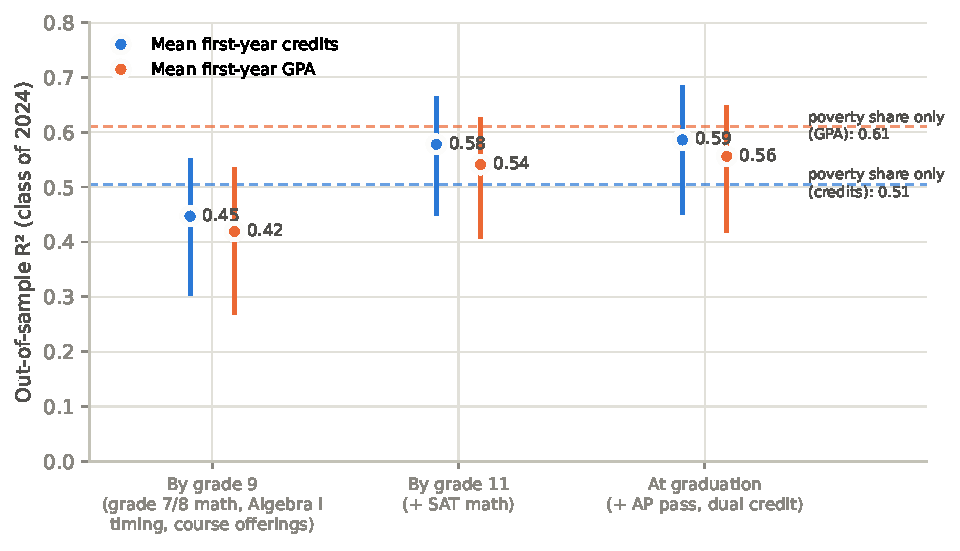
\includegraphics[width=0.92\linewidth]{figures/fig1_information_tiers.pdf}
\caption{Out-of-sample $R^2_w$ for the class of 2024 by the information available at three points in the cohort's high school career. Bars are 95\% corporation-cluster bootstrap intervals. Dashed lines: a model using only the school's FRL share.}\label{fig:tiers}
\end{figure}

\begin{table}[t]
\centering
\caption{Out-of-sample $R^2_w$ (class of 2024) by information tier, with 95\% cluster-bootstrap intervals.}\label{tab:tiers}
\small
\begin{tabular}{@{}lllll@{}}
\toprule
Information set & Mean credits & Mean GPA & $<$24 credits & GPA $<$ 2.0 \\
\midrule
By grade 9 & 0.45 [0.30, 0.55] & 0.42 [0.27, 0.54] & 0.49 & 0.32 \\
By grade 11 & 0.58 [0.45, 0.67] & 0.54 [0.41, 0.63] & 0.61 & 0.39 \\
At graduation & 0.59 [0.45, 0.69] & 0.56 [0.42, 0.65] & 0.61 & 0.40 \\
FRL share only & 0.51 & 0.61 & 0.52 & 0.49 \\
\bottomrule
\end{tabular}
\end{table}

\subsec{Calibration}
Predictions were well ordered but slightly too extreme (Figure~\ref{fig:calibration}). The calibration slope was 0.87 for credits (95\% CI 0.79--0.96) and 0.90 for GPA (0.81--1.00): schools predicted to do very well or very poorly ended up somewhat closer to the middle. The larger miss was in level. Statewide mean first-year credits rose from 23.0 to 23.6 between the classes of 2023 and 2024, and the model trained on 2023 under-predicted 2024 by 0.67 credits on average (CITL); for GPA the level error was 0.042. A common shift does not change which schools are flagged, but a model used for absolute targets needs its intercept updated each year from the latest statewide figure, and a slope below one argues for shrinking extreme predictions toward the mean.

\begin{figure}[t]
\centering
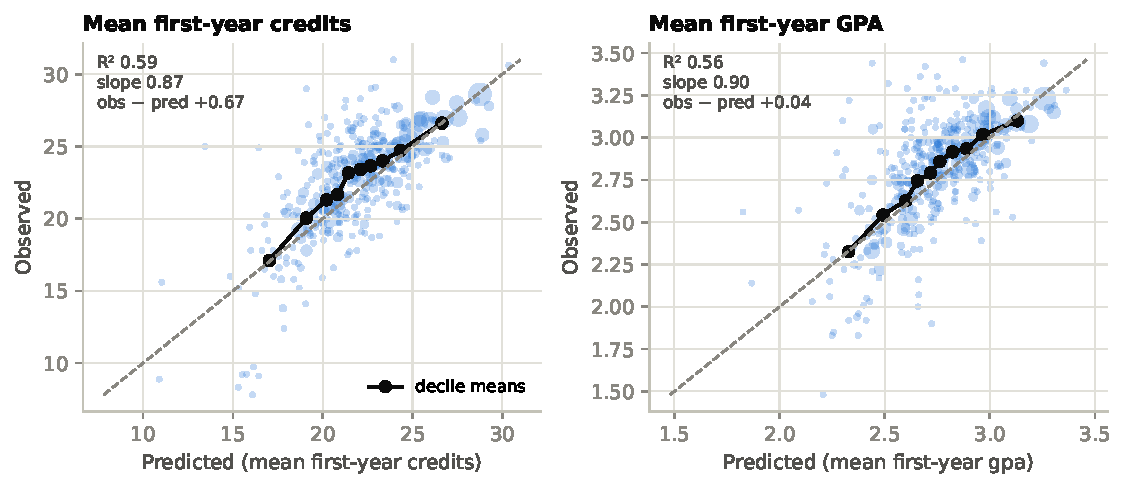
\includegraphics[width=\linewidth]{figures/fig2_calibration.pdf}
\caption{Observed versus predicted outcomes, class of 2024 (model fit on 2023). Points are schools (area proportional to enrollees); black points are enrollee-weighted decile means; the dashed line is perfect calibration.}\label{fig:calibration}
\end{figure}

\subsec{Drift across cohorts}
Without SAT, accuracy decays slowly with distance from the training cohort (Figure~\ref{fig:drift}, Table~\ref{tab:drift}). Trained on the class of 2021, the model explained 52\%, 51\% and 42\% of credits for 2022, 2023 and 2024, and its CITL grew from 0.62 to 1.19 credits as statewide outcomes improved. Pooling 2021 and 2022 raised accuracy for 2023 and 2024 (57\% and 51\%). Backcasting from 2023 to 2021 was weakest (32\%), plausibly because the class of 2021's first college year fell in 2021--22, under pandemic conditions. These results argue for refitting each year on the two most recent cohorts.

\begin{figure}[t]
\centering
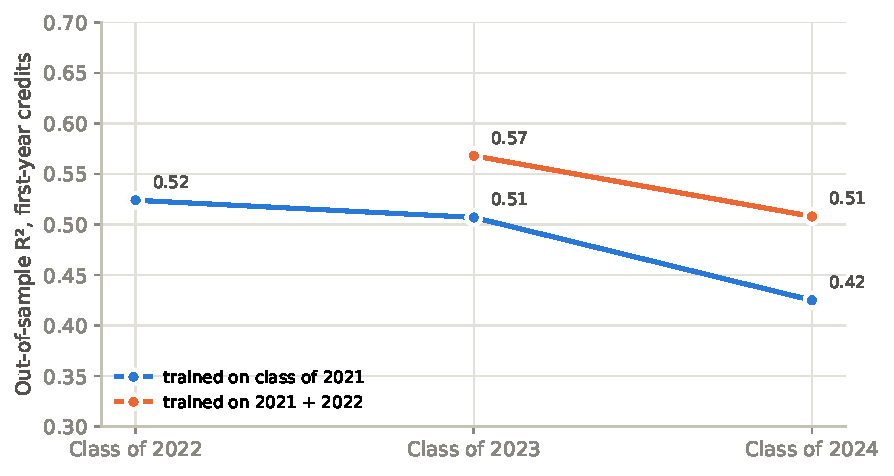
\includegraphics[width=0.82\linewidth]{figures/fig3_cohort_drift.pdf}
\caption{Out-of-sample $R^2_w$ for mean first-year credits when the reduced lever set (no SAT) is applied to later cohorts.}\label{fig:drift}
\end{figure}

\begin{table}[t]
\centering
\caption{Cohort drift with the reduced lever set (no SAT). Slope is the calibration slope; CITL is mean observed minus predicted.}\label{tab:drift}
\small
\begin{tabular}{@{}llrrrrrr@{}}
\toprule
 & & \multicolumn{3}{c}{Mean credits} & \multicolumn{2}{c}{Mean GPA} & $<$24 cr. \\
\cmidrule(lr){3-5}\cmidrule(lr){6-7}\cmidrule(l){8-8}
Trained on & Test & $R^2_w$ & Slope & CITL & $R^2_w$ & CITL & $R^2_w$ \\
\midrule
Class of 2021 & 2022 & 0.52 & 1.21 & +0.62 & 0.42 & +0.063 & 0.53 \\
 & 2023 & 0.51 & 1.12 & +0.76 & 0.38 & +0.080 & 0.50 \\
 & 2024 & 0.42 & 0.97 & +1.19 & 0.35 & +0.099 & 0.52 \\
Classes of 2021--2022 & 2023 & 0.57 & 1.06 & +0.38 & 0.46 & +0.042 & 0.56 \\
 & 2024 & 0.51 & 0.91 & +0.79 & 0.44 & +0.060 & 0.57 \\
Class of 2023 & 2021 & 0.32 & 0.70 & -0.58 & 0.25 & -0.060 & 0.29 \\
 & 2022 & 0.55 & 0.89 & +0.15 & 0.43 & +0.012 & 0.57 \\
 & 2024 & 0.54 & 0.84 & +0.36 & 0.47 & +0.013 & 0.57 \\
\bottomrule
\end{tabular}
\end{table}

\subsec{Warning flags}
Flagging the fifth of schools with the lowest predicted credits identified 46 of the 75 schools that turned out to be in the lowest fifth (Table~\ref{tab:flags}): precision 62\% and recall 61\%, against 20\% by chance and 55\% for the persistence flag. For the off-track share the model's precision was 60\% against 52\% for persistence; for GPA the two were similar. About two in five flagged schools are therefore not in the worst fifth when outcomes arrive, which is why the flag should prompt closer review rather than serve as a rating.

\begin{table}[t]
\centering
\caption{Worst-fifth warning flags for the class of 2024. Chance precision is 0.20.}\label{tab:flags}
\small
\begin{tabular}{@{}lrrrrr@{}}
\toprule
Outcome & Flagged & Truly worst & Hits & Precision (recall) & Persistence precision \\
\midrule
Mean credits (lowest fifth) & 74 & 75 & 46 & 0.62 (0.61) & 0.55 \\
Mean GPA (lowest fifth) & 74 & 74 & 44 & 0.59 (0.59) & 0.59 \\
Share $<$24 credits (highest fifth) & 74 & 74 & 44 & 0.59 (0.59) & 0.52 \\
Share GPA $<$2.0 (highest fifth) & 74 & 78 & 41 & 0.55 (0.53) & 0.54 \\
\bottomrule
\end{tabular}
\end{table}

\subsec{Which levers carry the signal}
Table~\ref{tab:levers} and Figure~\ref{fig:levers} report the coefficients from the linear model on the classes of 2023 and 2024 pooled. Holding the other levers fixed, grade 11 SAT mathematics dominated: one standard deviation corresponded to 1.97 more first-year credits (95\% CI 1.55--2.32) and 0.19 GPA points. The share of graduates earning dual credit was the only other lever whose interval excluded zero for both outcomes (0.36 credits; 0.050 GPA). Grade 7/8 mathematics, Algebra~I timing and course offerings were strongly related to outcomes on their own (in 2024 the correlation of credits with the late Algebra~I share was -0.41, with grade 7/8 mathematics 0.43 and with calculus offered 0.31) but added little once SAT mathematics was known. SAT alone explained 57\% of credits and grade 7/8 mathematics alone 41\%; dropping SAT from the full model lowered $R^2_w$ to 54\%. The early signals' information about a cohort is largely carried forward into its grade 11 results. These are cross-school associations: they indicate where to look, not what would happen if a school changed one lever.

\begin{table}[t]
\centering
\caption{Lever coefficients: change in the outcome per one standard deviation of each lever, classes of 2023--2024 pooled, with 95\% corporation-cluster bootstrap intervals. $^{*}$Interval excludes zero.}\label{tab:levers}
\small
\begin{tabular}{@{}lrlrl@{}}
\toprule
Lever & \multicolumn{2}{c}{Mean credits} & \multicolumn{2}{c}{Mean GPA} \\
\midrule
Grade 11 SAT math benchmark rate & 1.97$^{*}$ & [1.55, 2.32] & 0.194$^{*}$ & [0.146, 0.229] \\
Graduates earning dual credit & 0.36$^{*}$ & [0.16, 0.58] & 0.050$^{*}$ & [0.016, 0.081] \\
Graduates passing an AP exam & 0.22 & [-0.02, 0.45] & -0.025 & [-0.056, 0.002] \\
Offers calculus & 0.12 & [-0.09, 0.33] & 0.008 & [-0.015, 0.031] \\
Offers advanced mathematics & 0.07 & [-0.16, 0.27] & 0.004 & [-0.014, 0.026] \\
Algebra I passers in grades 9--12 per student & 0.03 & [-0.11, 0.19] & 0.012 & [-0.011, 0.035] \\
Grade 7/8 math proficiency ($z$) & -0.10 & [-0.32, 0.19] & 0.003 & [-0.027, 0.036] \\
Advanced math + calculus enrollment share & -0.12 & [-0.32, 0.07] & -0.016 & [-0.033, 0.003] \\
Algebra I passed in grades 11--12 (share) & -0.14 & [-0.45, 0.05] & -0.002 & [-0.024, 0.024] \\
\bottomrule
\end{tabular}
\end{table}

\begin{figure}[t]
\centering
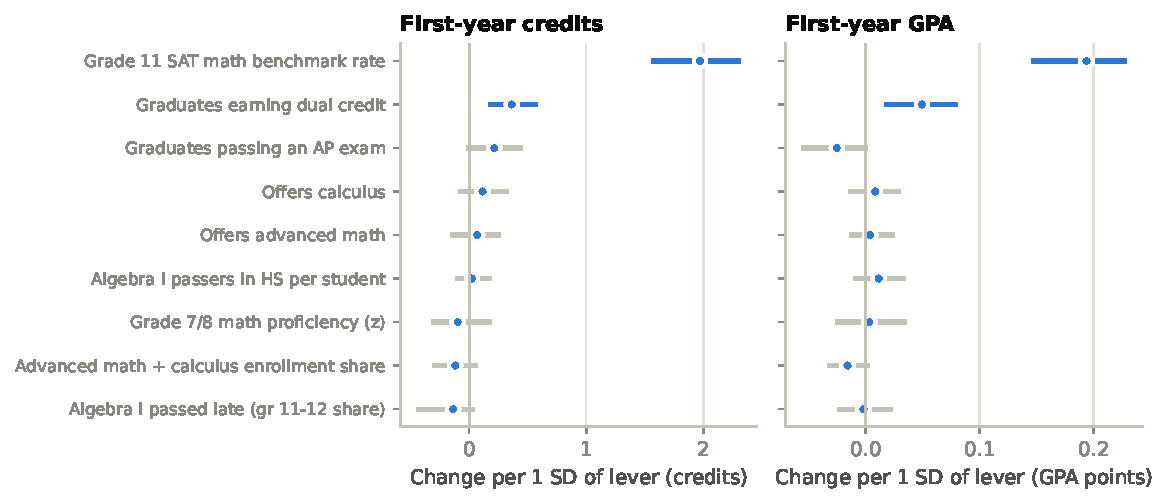
\includegraphics[width=\linewidth]{figures/fig4_levers.pdf}
\caption{Lever coefficients per one standard deviation, with 95\% cluster-bootstrap intervals; gray intervals cross zero.}\label{fig:levers}
\end{figure}

\subsec{Where the model fails}
Net of the statewide shift, most group residuals were small (Table~\ref{tab:audit}, Figure~\ref{fig:audit}), but several departures were consistent. The model under-predicted GPA at small schools (0.06 points), rural schools (0.03) and junior/senior high schools whose own grade 8 results were used (0.07; also 0.67 credits), and over-predicted GPA at high-poverty schools (-0.04). The seven virtual schools were under-predicted by 0.28 GPA points. Charter schools were over-predicted on average (-1.01 credits) with large dispersion. The 20 worst-predicted schools were dominated by small schools (18 of 20 had fewer than 30 enrollees) and over-represented charter and virtual schools (8 of 20, against 11\% of schools overall). The over-prediction at high-poverty schools matters most for use: the levers alone slightly understate the disadvantage these graduates face in college, so a lever-based flag will miss some of the schools most in need.

\begin{table}[t]
\centering
\caption{Failure audit, class of 2024 (model fit on 2023). Mean residual is observed minus predicted, net of the statewide shift; positive values mean the group did better than predicted. $^{*}|t|>2$.}\label{tab:audit}
\small
\begin{tabular}{@{}llrrrrr@{}}
\toprule
 & & & \multicolumn{2}{c}{Mean credits} & \multicolumn{2}{c}{Mean GPA} \\
\cmidrule(lr){4-5}\cmidrule(l){6-7}
Grouping & Level & Schools & Mean resid. & RMSE & Mean resid. & RMSE \\
\midrule
Locale & City & 74 & -0.19 & 1.74 & -0.042 & 0.198 \\
 & Rural & 165 & +0.20 & 2.36 & +0.034$^{*}$ & 0.208 \\
 & Suburb & 64 & -0.09 & 1.37 & -0.003 & 0.124 \\
 & Town & 64 & +0.28 & 2.15 & +0.035 & 0.191 \\
\addlinespace
Poverty tercile (FRL) & low FRL & 123 & -0.16 & 1.60 & +0.006 & 0.136 \\
 & middle FRL & 122 & +0.16 & 1.95 & +0.034 & 0.219 \\
 & high FRL & 122 & +0.14 & 2.14 & -0.036$^{*}$ & 0.200 \\
\addlinespace
Size tercile (enrollees) & small & 128 & +0.17 & 3.41 & +0.063$^{*}$ & 0.354 \\
 & medium & 120 & +0.03 & 2.17 & -0.000 & 0.191 \\
 & large & 120 & -0.03 & 1.43 & -0.008 & 0.134 \\
\addlinespace
School type & charter & 32 & -1.01 & 3.93 & -0.121 & 0.378 \\
 & traditional & 329 & +0.04 & 1.73 & -0.001 & 0.161 \\
 & virtual & 7 & -0.61 & 3.26 & +0.283$^{*}$ & 0.435 \\
\addlinespace
Grade 8 data attributed to & district average & 249 & -0.02 & 1.64 & -0.005 & 0.149 \\
 & own building & 97 & +0.67$^{*}$ & 2.89 & +0.070$^{*}$ & 0.298 \\
\addlinespace
Only high school in district & no & 93 & -0.27 & 1.69 & -0.029 & 0.157 \\
 & yes & 275 & +0.13 & 1.94 & +0.014 & 0.187 \\
\bottomrule
\end{tabular}
\end{table}

\begin{figure}[t]
\centering
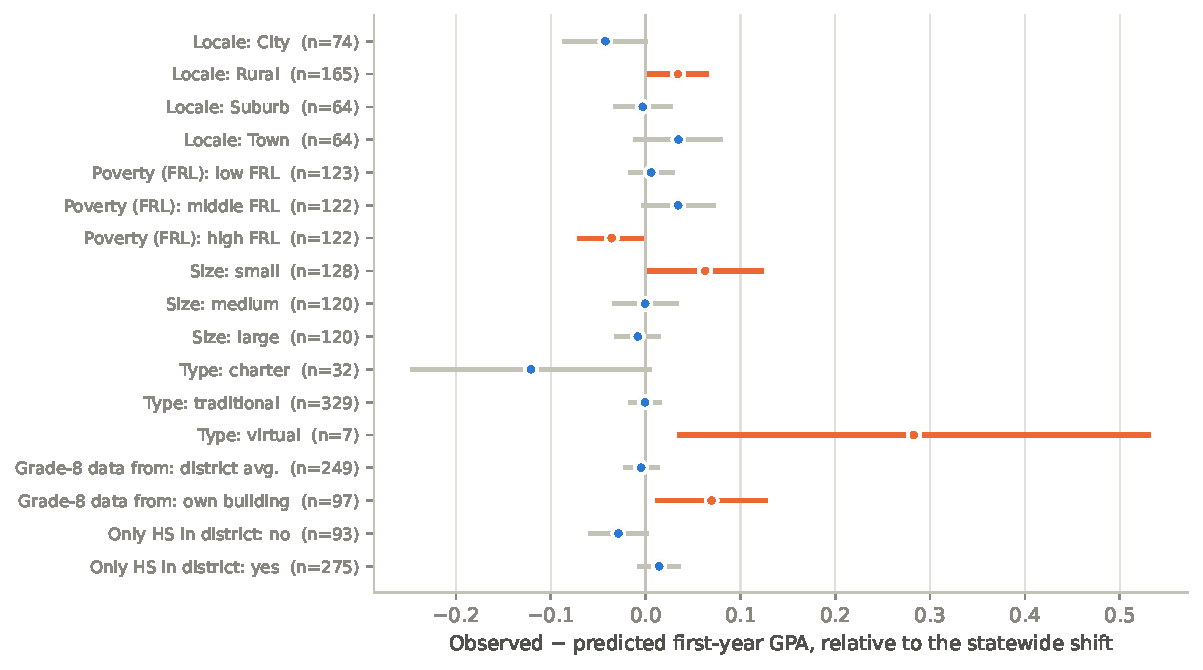
\includegraphics[width=0.9\linewidth]{figures/fig5_failure_audit.pdf}
\caption{Mean GPA residual (observed minus predicted, net of the statewide shift) by school group, class of 2024. Bars are $\pm 2$ standard errors; orange marks $|t|>2$.}\label{fig:audit}
\end{figure}

\subsec{Sensitivity analyses}
Table~\ref{tab:sens} collects the sensitivity checks. Adding FRL share to the model raised $R^2_w$ to 0.60 for credits and 0.63 for GPA. Restricting to the 235 schools with at least 30 enrollees raised it to 0.61 and 0.64, confirming that much of the remaining error is sampling noise in small schools.

\begin{table}[t]
\centering
\caption{Sensitivity of out-of-sample $R^2_w$ (class of 2024, fit on 2023).}\label{tab:sens}
\small
\begin{tabular}{@{}lrr@{}}
\toprule
Specification & Mean credits & Mean GPA \\
\midrule
Full lever set (headline) & 0.59 & 0.56 \\
Full lever set + FRL share & 0.60 & 0.63 \\
Full lever set without SAT & 0.54 & 0.47 \\
SAT mathematics only & 0.57 & 0.52 \\
Grade 7/8 mathematics only & 0.41 & 0.41 \\
FRL share only & 0.51 & 0.61 \\
Schools with $\ge$30 enrollees (n = 235) & 0.61 & 0.64 \\
\bottomrule
\end{tabular}
\end{table}

\subsec{Mathematics remediation}
Remediation shares are published for only 141 of the 368 schools in the class-of-2024 sample, and remediation is rare: 4.2\% of Indiana public college enrollees needed mathematics remediation in 2024, compared with 4.9\% in 2021. Among reporting schools, the remediation share was essentially uncorrelated with predicted credits ($r = 0.03$) and with SAT mathematics ($r = -0.03$). We read this as a measurement result: with suppression and low prevalence, the published remediation field cannot support school-level modeling, and first-year credits and GPA are the better-measured indicators of how graduates fare in college mathematics-dependent coursework.

\section{Discussion}\label{sec:discussion}

Public school-level signals predict roughly three-fifths of the between-school variation in first-year college credits and GPA for a cohort the model has not seen, and most of that warning is available by grade~11. A weighted linear model does as well as a tree ensemble, beats waiting for the previous cohort's outcomes, and its errors can be described in plain terms. For a district, the practical reading is that a high school whose grade 11 SAT mathematics results and dual-credit participation are low relative to the state should expect its graduates to accumulate credits slowly in college, two or more years before the state reports it. For the state, the model offers a way to direct attention to schools before outcomes are observed, provided the flag is treated as a starting point for review.

Three findings temper that use. First, a school's poverty rate predicts GPA as well as the lever set. The levers partly proxy the same disadvantage, and the model slightly over-predicts how graduates of high-poverty schools fare; adding poverty improves accuracy but turns the tool toward describing demographics rather than practice. We report it as a sensitivity analysis and leave the choice to users, but any use of flags for resource allocation should check whether they simply track poverty. Second, lever coefficients are associations. The late-Algebra~I share and course offerings are strongly related to outcomes but add little once SAT is known. This is consistent with a pathway in which early mathematics shapes grade 11 performance, and with the evidence that acceleration alone does not raise later achievement \citep{clotfelter2015,domina2015}, but cross-school data cannot establish it. Third, the model is weakest exactly where small numbers make every school-level statistic noisy: small, rural, charter and virtual schools.

\subsec{Limitations}
Outcomes cover only graduates who enrolled at an Indiana public college, about 36\% of the class of 2024 statewide; graduates at private or out-of-state colleges are not observed, and enrollment selection differs across schools. Grade 8 results are attributed through the school corporation for most high schools, which blurs differences within multi-high-school districts, and the class of 2024 uses grade 7 results because the 2020 test was cancelled. State SAT exists only from the class of 2023, so the full model rests on a single cohort transition. CRDC data are biennial and self-reported, and Algebra~I timing is observed only within the high school building. Earlier CHE files were linked by school name, and renamed schools may drop from earlier cohorts. The FRL measure used in the audit is affected by community-eligibility reporting. Finally, the model is school-level and must not be used for decisions about individual students \citep{robinson1950}.

\subsec{Next steps}
The most important extension is prospective: publishing predictions for the classes of 2025 and 2026, whose grade 8 and grade 11 results already exist, and scoring them when CHE releases their outcomes in 2027 and 2028. Further work should replace corporation-average grade 8 attribution with feeder-school weights, add the full 2023--24 CRDC, validate flags against district knowledge, and test whether the same levers predict second-year persistence.

\section{Conclusion}\label{sec:conclusion}

An early, transparent and calibrated school-level warning of weak first-year college outcomes is feasible for Indiana from public data alone. It is most informative by grade~11, it does not need a black box, and its failures are concentrated in small, rural, high-poverty and nontraditional schools. The panel, code, model card and an interactive school map are released so that districts and the state can test the warnings against what they know and refit the model as each new cohort's outcomes are published. The project is available at \url{https://github.com/OthnyLight/in-hs-math-earlywarning}.

\subsec{Data and code availability}
All inputs are public. The derived panel, predictions, statistics file, figures and code are available at \url{https://github.com/OthnyLight/in-hs-math-earlywarning} under CC BY 4.0 (data and text) and MIT (code). Raw-file hashes are recorded in \code{data/raw/PROVENANCE.txt}.

\subsec{Use of AI tools}
An AI assistant (Anthropic's Claude) was used to write data-processing and modeling code, draft text and produce figures under the author's direction. The author specified the research questions, made the analytic decisions, reproduced the pipeline, checked the numbers against the source files and is responsible for the content.

\subsec{Funding and competing interests}
None. The author declares no competing interests.

\renewcommand{\refname}{Bibliography}
\section*{Bibliography}
\begingroup\small
\renewcommand{\section}[2]{}
\begin{thebibliography}{99}
\setlength{\itemsep}{0.55ex}

\bibitem[Adelman(2006)]{adelman2006} C.~Adelman. \emph{The Toolbox Revisited: Paths to Degree Completion from High School through College}. U.S. Department of Education, Washington, DC, 2006.

\bibitem[Allensworth and Easton(2005)]{allensworth2005} E.~M. Allensworth and J.~Q. Easton. \emph{The On-Track Indicator as a Predictor of High School Graduation}. Consortium on Chicago School Research, University of Chicago, 2005.

\bibitem[An(2013)]{an2013} B.~P. An. The impact of dual enrollment on college degree attainment: Do low-SES students benefit? \emph{Educational Evaluation and Policy Analysis}, 35(1):57--75, 2013.

\bibitem[Bailey et~al.(2010)]{bailey2010} T.~Bailey, D.~W. Jeong, and S.-W. Cho. Referral, enrollment, and completion in developmental education sequences in community colleges. \emph{Economics of Education Review}, 29(2):255--270, 2010.

\bibitem[Bowers et~al.(2013)]{bowers2013} A.~J. Bowers, R.~Sprott, and S.~A. Taff. Do we know who will drop out? A review of the predictors of dropping out of high school: Precision, sensitivity, and specificity. \emph{The High School Journal}, 96(2):77--100, 2013.

\bibitem[Cameron et~al.(2008)]{cameron2008} A.~C. Cameron, J.~B. Gelbach, and D.~L. Miller. Bootstrap-based improvements for inference with clustered errors. \emph{The Review of Economics and Statistics}, 90(3):414--427, 2008.

\bibitem[Clotfelter et~al.(2015)]{clotfelter2015} C.~T. Clotfelter, H.~F. Ladd, and J.~L. Vigdor. The aftermath of accelerating algebra: Evidence from district policy initiatives. \emph{Journal of Human Resources}, 50(1):159--188, 2015.

\bibitem[Collins et~al.(2015)]{collins2015} G.~S. Collins, J.~B. Reitsma, D.~G. Altman, and K.~G.~M. Moons. Transparent reporting of a multivariable prediction model for individual prognosis or diagnosis (TRIPOD): The TRIPOD statement. \emph{Annals of Internal Medicine}, 162(1):55--63, 2015.

\bibitem[Cox(1958)]{cox1958} D.~R. Cox. Two further applications of a model for binary regression. \emph{Biometrika}, 45(3--4):562--565, 1958.

\bibitem[Domina et~al.(2015)]{domina2015} T.~Domina, A.~McEachin, A.~Penner, and E.~Penner. Aiming high and falling short: California's eighth-grade algebra-for-all effort. \emph{Educational Evaluation and Policy Analysis}, 37(3):275--295, 2015.

\bibitem[Efron and Tibshirani(1993)]{efron1993} B.~Efron and R.~J. Tibshirani. \emph{An Introduction to the Bootstrap}. Chapman \& Hall, New York, 1993.

\bibitem[Eilers and Marx(1996)]{eilers1996} P.~H.~C. Eilers and B.~D. Marx. Flexible smoothing with B-splines and penalties. \emph{Statistical Science}, 11(2):89--121, 1996.

\bibitem[Friedman(2001)]{friedman2001} J.~H. Friedman. Greedy function approximation: A gradient boosting machine. \emph{The Annals of Statistics}, 29(5):1189--1232, 2001.

\bibitem[Indiana Commission for Higher Education(2026)]{che2026} Indiana Commission for Higher Education. College-going and college-readiness datasets, high school graduating classes of 2021--2024, 2023--2026. URL \url{https://www.in.gov/che/college-going-reports/}.

\bibitem[Long et~al.(2009)]{long2009} M.~C. Long, P.~Iatarola, and D.~Conger. Explaining gaps in readiness for college-level math: The role of high school courses. \emph{Education Finance and Policy}, 4(1):1--33, 2009.

\bibitem[Mitchell et~al.(2019)]{mitchell2019} M.~Mitchell, S.~Wu, A.~Zaldivar, P.~Barnes, L.~Vasserman, B.~Hutchinson, E.~Spitzer, I.~D. Raji, and T.~Gebru. Model cards for model reporting. In \emph{Proceedings of the Conference on Fairness, Accountability, and Transparency}, pages 220--229, 2019.

\bibitem[Pedregosa et~al.(2011)]{pedregosa2011} F.~Pedregosa, G.~Varoquaux, A.~Gramfort, et~al. Scikit-learn: Machine learning in Python. \emph{Journal of Machine Learning Research}, 12:2825--2830, 2011.

\bibitem[Robinson(1950)]{robinson1950} W.~S. Robinson. Ecological correlations and the behavior of individuals. \emph{American Sociological Review}, 15(3):351--357, 1950.

\bibitem[Scott-Clayton(2012)]{scottclayton2012} J.~Scott-Clayton. Do high-stakes placement exams predict college success? CCRC Working Paper 41, Community College Research Center, Teachers College, Columbia University, 2012.

\bibitem[Steyerberg(2019)]{steyerberg2019} E.~W. Steyerberg. \emph{Clinical Prediction Models: A Practical Approach to Development, Validation, and Updating}. Springer, Cham, 2nd edition, 2019.

\bibitem[Urban Institute(2026)]{urban2026} Urban Institute. Education Data Portal: Civil Rights Data Collection and Common Core of Data endpoints, 2026. URL \url{https://educationdata.urban.org/}. Accessed 9 October 2026.

\bibitem[Van~Calster et~al.(2019)]{vancalster2019} B.~Van~Calster, D.~J. McLernon, M.~van Smeden, L.~Wynants, and E.~W. Steyerberg. Calibration: The Achilles heel of predictive analytics. \emph{BMC Medicine}, 17:230, 2019.
\end{thebibliography}
\endgroup

\vspace{3ex}
\noindent\begin{minipage}{\linewidth}\small
\emph{Othniel Iyassa Sa'anga}\\
\emph{Independent Researcher}\\
\emph{ORCiD:} \href{https://orcid.org/0009-0002-6113-6158}{\color{linkblue}\emph{0009-0002-6113-6158}}\\
{\color{linkblue}\texttt{othnylight@gmail.com}}
\end{minipage}

\end{document}
